\chapter{Approximate Bayesian methods}\label{chap15}

\textit{Approximate Bayesian methods} are a family of techniques designed to handle situations where the likelihood function lacks an analytical expression, is highly complex, or the problem has high dimensionality, whether due to a large parameter space or a massive dataset \cite{martin2024approximating}. In the former case, traditional Markov Chain Monte Carlo (MCMC) and importance sampling algorithms fail to provide a solution, while in the latter, these algorithms struggle to produce accurate estimates within a reasonable time.  

However, there is no free lunch, \textit{Approximate Bayesian methods} address these challenges at the cost of providing an approximation to the posterior distribution rather than the \textit{exact} posterior. Nonetheless, asymptotic results show that the approximation improves as the sample size increases.

In this chapter, I first present \textit{simulation-based approaches}, which are designed to address situations where the likelihood is highly complex and may lack an analytical solution. In the second part, I introduce \textit{optimization approaches}, which are intended to handle high-dimensional problems. Specifically, I discuss approximate Bayesian computation (ABC) and Bayesian synthetic likelihood (BSL), the two most common \textit{simulation-based approaches}. Then, I present integrated nested Laplace approximations (INLA) and \textit{variational Bayes} (VB), the two most common \textit{optimization approaches} for high-dimensional problems.

\section{Simulation-based approaches}\label{sec15_1}
Taking into account the fundamental equation for performing parameter inference in the Bayesian framework,  
\begin{align*}
	\pi(\boldsymbol{\theta} \mid \mathbf{y}) & \propto p(\mathbf{y} \mid \boldsymbol{\theta}) \times \pi(\boldsymbol{\theta}),
\end{align*}  
we see in Section \ref{sec51} that MCMC algorithms, such as the Gibbs sampler (Section \ref{sec511}) and Metropolis-Hastings (Section \ref{sec512}), require evaluation of the likelihood function \( p(\boldsymbol{y} \mid \boldsymbol{\theta}) \) in the posterior conditional distribution or the acceptance probability, respectively. This is also the case for importance sampling when calculating the importance weights (Section \ref{sec52}).  

Thus, what happens when the likelihood function does not have an analytical expression? This situation arises in many models involving unobserved heterogeneity (i.e., unobserved taste preferences), models defined by quantile functions (e.g., the g-and-k distribution), or dynamic equilibrium model (e.g., repeated game models).

\textit{Simulation-based algorithms} provide a Bayesian solution when we face this situation, namely, when the likelihood function lacks an analytical expression or is highly complex. The only requirement is that we must be able to simulate synthetic data from the model conditional on the parameters. Therefore, these algorithms obtain an approximation to the posterior draws by simulating from the prior distribution $\pi(\boldsymbol{\theta})$ and then using these draws to simulate from the likelihood $p(\mathbf{y} \mid \boldsymbol{\theta})$.

\subsection{Approximate Bayesian computation}\label{sec15_12}

\textit{Approximate Bayesian Computation} (ABC) is designed to handle inferential situations where the likelihood function \( p(\boldsymbol{y} \mid \boldsymbol{\theta}) \) is intractable or highly complex, $\boldsymbol{y}\in \mathbb{R}^N$. It was introduced in population genetics by \cite{tavare1997inferring, pritchard1999population} and later generalized by \cite{beaumont2002approximate}. The basic intuitive origin of ABC appears to have been introduced by \cite{rubin1984bayesianly}. A growing body of literature explores its applications in biology, cosmology, finance, economics, and other fields.

The requirement in ABC is the ability to simulate from the parametric model. The process begins by drawing samples from the prior distribution \( \pi({\boldsymbol{\theta}}) \) multiple times, $\boldsymbol{\theta}\in\mathbb{R}^K$, and then simulating data from the model given each \( {\boldsymbol{\theta}^{(s)}}, s=1,2,\dots,S \). The resulting synthetic data, \( \boldsymbol{z}^{(s)} \in \mathbb{R}^N \) is used to compute summary statistics \( \boldsymbol{\eta}(\boldsymbol{z}^{(s)}) \in \mathbb{R}^L, L\geq K \). These summary statistics are crucial for the performance of ABC and should be selected based on a thorough understanding of the model.  

Next, we compare the synthetic summary statistics with the observed summary statistics \( \boldsymbol{\eta}(\boldsymbol{y}) \) using a distance metric \( d\left\{ \boldsymbol\eta ({\boldsymbol y}),{\boldsymbol \eta }({\boldsymbol z}^{(s)})\right\} \), typically the Euclidean distance. We retain the prior draws that generate synthetic summary statistics closest to the observed ones, that is, \( d\left\{ \boldsymbol\eta ({\boldsymbol y}),{\boldsymbol \eta }({\boldsymbol z}^{(s)})\right\}\leq \epsilon \), forming an approximation of the posterior distribution \( \pi_{\epsilon}(\boldsymbol{\theta},\boldsymbol{z} \mid \boldsymbol{\eta}(\boldsymbol{y})) \).

The simplest algorithm is the accept/reject approximate Bayesian computation (ABC-AR) (see Algorithm \ref{ABC0}).

\begin{algorithm}
	\caption{Accept/reject ABC}\label{ABC0}
	\begin{algorithmic}[1]
		\For{\texttt{$s=1,\dots,S$}}
		\State Draw ${\boldsymbol {\theta} }^{s}$ from $\pi({ \boldsymbol{\theta} }),$
		\State Simulate ${\boldsymbol z}^{s}=(z_{1}^{s},z_{2}^{s},...,z_{n}^{s})^{\top}$ from the model, $p(\cdot|{\boldsymbol{\theta} }^{s})$
		\State Calculate
		$d_{(s)}=d\{{\boldsymbol\eta }({\boldsymbol y}),{\boldsymbol \eta }({\boldsymbol z}^{s})\}$
		\EndFor
		\State Order the distances $d_{(1)}\leq\cdots\leq d_{(S)}$
		\State Select all $\boldsymbol{\theta}^s$ such that $d_{(i)}\leq \epsilon$, where $\epsilon>0$ is the tolerance level. 
	\end{algorithmic}
\end{algorithm}

Note that the posterior distribution is conditional on the summary statistics \( \boldsymbol{\eta}(\boldsymbol{y}) \) and the tolerance parameter \( \epsilon \). This implies that we obtain an approximation to the target distribution \( \pi(\boldsymbol{\theta} \mid \boldsymbol{y}) \), that is \( \pi(\boldsymbol{\theta} \mid \boldsymbol{\eta}(\boldsymbol{y})) \), because \( \boldsymbol{\eta}(\boldsymbol{y}) \) is not a sufficient statistic in most cases, and \( \epsilon > 0 \), these conditions introduce bias \cite{blum2010approximate}. However, ABC performs well compared to full-likelihood approaches in low-dimensional parameter spaces \cite{beaumont2002approximate}.

Furthermore, \cite{frazier2018asymptotic} show in Theorems 1 and 2 that Bayesian consistency and asymptotic normality hold, provided that \( \epsilon \to 0 \) fast enough as \( n \to +\infty \). In particular, the requirement is that the proportion of accepted draws converges to 0 at a rate faster than \( n^{-K / 2} \). Additionally, Theorem 2 in \cite{frazier2018asymptotic} shows that \( 100(1 -\alpha)\% \) Bayesian credible regions using ABC have frequentist coverage of \( 100(1 -\alpha)\% \). 

We should note from these asymptotic results that ABC suffers from the \textit{curse of dimensionality}. Specifically, given a sample size of 1,000 and two parameters, the proportion of accepted draws should be 0.1\%, meaning we would require one million prior draws to obtain 1,000 posterior draws. On the other hand, if the number of parameters is three, we would require 31.62 million prior draws. This limitation of ABC has attracted attention; see Chapter 8 of \cite{sisson2018handbook} for some potential solutions.

It is a common practice in ABC to perform a regression adjustment after retaining the draws \cite{beaumont2002approximate, leuenberger2010bayesian, sisson2018handbook}. This adjustment reduces bias in posterior draws by performing a simple linear regression between the selected draws and the discrepancy between the observed and simulated summary statistics, \( {\theta}^{(s)}_k = \alpha_k + \left(\boldsymbol{\eta}(\boldsymbol{y}) - \boldsymbol{\eta}(\boldsymbol{z}^{(s)})\right)^{\top}\boldsymbol{\beta}_k + \mu^{(s)}_k, \ k=1,2,\dots,K \). Then, the posterior draws are adjusted using the slope estimate \( {\theta}^{\text{adj},(s)}_k = {\theta}^{(s)}_k - \left(\boldsymbol{\eta}(\boldsymbol{y}) - \boldsymbol{\eta}(\boldsymbol{z}^{(s)})\right)^{\top}\hat{\boldsymbol{\beta}}_k \). Other regression adjustment strategies are also used, such as local linear regression, ridge regression, and neural networks. See the \textit{abc} package in \textbf{R}.

The favorable asymptotic sampling properties of ABC rely on correct model specification. \cite{frazier2020model} demonstrate that when the assumed model is misspecified, the asymptotic behavior of ABC can deteriorate. In particular, the posterior shape becomes asymptotically non-Gaussian, and the behavior of the posterior mean remains generally unknown. Additionally, regression adjustment approaches can produce posteriors that differ significantly from their simpler accept/reject counterparts.

Given these concerns, testing model specification in ABC is essential. This can be done using simulated goodness-of-fit statistics \cite{bertorelle2010abc,lintusaari2017fundamentals}, predictive p-values \cite{bertorelle2010abc}, discrepancy diagnostics \cite{frazier2020model}, and asymptotic tests \cite{ramirez2024testing} to evaluate model adequacy.

The accept/reject ABC algorithm is inefficient, as all draws are independent; thus, there is no learning from previous draws. This intensifies the computational burden. Therefore, \cite{marjoram2003markov, wegmann2009efficient} introduced Markov Chain Monte Carlo ABC (ABC-MCMC) algorithms, and \cite{sisson2007sequential, drovandi2011estimation, del2012adaptive, lenormand2013adaptive} proposed sequential Monte Carlo approaches (ABC-SMC). However, results comparing ABC-MCMC and ABC-SMC with ABC-AR are controversial regarding computational efficiency \cite{bertorelle2010abc}. In addition, ABC-AR is very simple and easily allows parallel computing \cite{frazier2019approximate}. Nevertheless, ABC-SMC is now the recommended approach, as it does not require tuning the algorithm's tolerance \cite{martin2024approximating}, and there are open-source implementations that facilitate its use.

New developments in ABC have focused on using empirical measures calculated from the observed ($\hat{\mu}_n$) and synthetic ($\hat{\mu}_{\boldsymbol{\theta}}^{(s)}$) data to replace summary statistics. Thus, $d\left\{ \boldsymbol\eta ({\boldsymbol y}),{\boldsymbol \eta }({\boldsymbol z}^{(s)})\right\}$ is replaced by $\mathcal{D}\left\{ \hat{\mu}_n,\hat{\mu}_{\boldsymbol{\theta}}^{(s)}\right\}$, where the latter is a discrepancy measure, such as the Kullback-Leibler divergence \cite{jiang2018approximate}. However, \cite{drovandi2022comparison} found in their simulation exercises that the best-performing summary statistics approach performs at least as well as the best discrepancy-measure approaches. The key point is to select informative summary statistics.\\

\textbf{Example: g-and-k distribution for financial returns} 

The g-and-k distribution is a highly flexible distribution capable of capturing skewness and heavy tails through its parameters. This makes it particularly useful for modeling real-world data that deviate from normality, especially in fields like finance, where outliers are common. However, this distribution lacks a closed-form expression for its density function.

The g-and-k distribution is defined by its quantile function \cite{drovandi2011likelihood}. Specifically, it is specified through its inverse cumulative distribution function,

\[
Q(p\mid{\theta}) = F^{-1}(p\mid{\theta}),
\]

where \( F = P(U \leq u) \), and \( Q \) represents the \( p \)-quantile \cite{rayner2002numerical}. The quantile function of the g-and-k distribution is given by

\[
Q^{gk}\left\{z(p)\mid a, b, c, g, k\right\} = a + b\left[1 + c \frac{1 - \exp\left\{-gz(p)\right\}}{1 + \exp\left\{-gz(p)\right\}}\right] \left\{1 + z(p)^2\right\}^k z(p),
\]

where \( z(p) \) is the standard normal quantile function, and \( c = 0.8 \) is a commonly suggested value.

In the g-and-k distribution, \( a \) is the location parameter, and \( b \) is the scale parameter, controlling the dispersion. The parameters \( g \) and \( k \) determine the levels of skewness and kurtosis, respectively, while \( c \) modifies the impact of skewness, and is typically set to 0.8.

\cite{drovandi2011likelihood} propose a moving average of order one using a g-and-k distribution to model exchange rate log returns. In particular,  
\[
z_t = \epsilon_t + \theta_1\epsilon_{t-1}, \quad t=1,\dots,524,
\]  
where \(\epsilon_t \sim N(0,1)\).  

The values of \(z_t\) are then divided by \((1+\theta_1^2)^{1/2}\) to ensure that they marginally follow a standard normal distribution. Thus, simulating g-and-k data requires only substituting \(z_t\) into the quantile function.  

We model exchange rate log daily returns from USD/EUR one year before and after the WHO declared the COVID-19 pandemic on 11 March 2020. We use the dataset \textit{ExchangeRate.csv} from our GitHub repository. Our ABC implementation uses twelve summary statistics: the seven octiles, the interquartile range, robust measures of skewness and kurtosis, and the autocorrelations of order one and two (see \cite{drovandi2011likelihood} and code below). We adopt the prior distributions proposed by \cite{ramirez2024testing}, 
\begin{align*}
	\theta_1\sim U(-1,1), \ a\sim U(0,5) \ b\sim U(0,5)\\
	g\sim U(-5,5), \ k\sim U(-0.5, 5).
\end{align*}

We use the \textit{EasyABC} package in \textbf{R} to implement the ABC accept/reject (ABC-AR) algorithm using 150,000 prior draws with an acceptance rate of 0.67\%. We also apply the ABC Markov chain Monte Carlo (ABC-MCMC) method \cite{marjoram2003markov} and the sequential Monte Carlo ABC (ABC-SMC) method \cite{lenormand2013adaptive} to compare the results across different ABC algorithms.\footnote{Note that this setting does not satisfy the asymptotic requirements for Bayesian consistency. However, it serves as a pedagogical exercise.} We generate 100,000 samples and retain 1\% in ABC-MCMC, and 30,000 samples, keeping 3.4\%, with a stopping criterion of 5\% in ABC-SMC. These settings imply that the three algorithms require approximately the same computational time. Users can refer to the cited references for algorithmic details.

In Exercise 1, we ask to program the ABC accept/reject algorithm (Algorithm \ref{ABC0}) from scratch and compare the results with those obtained using the ABC-AR implementation in the \textit{EasyABC} package.

The following code presents the results, and Figure \ref{figABCexc} compares the posterior distributions of $\theta_1$, $g$, and $k$ using the three methods. In this figure, we observe that ABC-MCMC (red) and ABC-SMC (green) exhibit similar performance, and both approaches provide more information than ABC-AR (blue). There is marginal positive evidence that the moving average coefficient is positive, and the three algorithms yield similar means, although ABC-AR exhibits lower precision. Since the posterior distribution of $g$ is centered around zero, the distribution appears to be symmetric around its median. Meanwhile, a positive $k$ indicates that the distribution has heavier tails than a normal distribution, implying a higher likelihood of extreme values (outliers) in the exchange rate USD/EURO.

\begin{tcolorbox}[enhanced,width=4.67in,center upper,
	fontupper=\large\bfseries,drop shadow southwest,sharp corners]
	\textit{R code. Exchange rate log returns: Approximate Bayesian computation}
	\begin{VF}
		\begin{lstlisting}[language=R]
######### ABC Exchange rate og returns: USD/EURO
rm(list = ls()); set.seed(010101)
library(EasyABC)
dfExcRate <- read.csv(file = "https://raw.githubusercontent.com/BEsmarter-consultancy/BSTApp/refs/heads/master/DataApp/ExchangeRate.csv", sep = ",", header = T)
attach(dfExcRate); n <- length(USDEUR)
# Summary statistics
SumSt <- function(y) {
	Oct <- quantile(y, c(0.125, 0.25, 0.375, 0.5, 0.625, 0.75, 0.875))
	eta1 <- Oct[6] - Oct[2]
	eta2 <- (Oct[6] + Oct[2] - 2 * Oct[4]) / eta1
	eta3 <- (Oct[7] - Oct[5] + Oct[3] - Oct[1]) / eta1
	autocor <- acf(y, lag = 2, plot = FALSE)
	autocor[["acf"]][2:3]
	Etay <- c(Oct, eta1, eta2, eta3, autocor[["acf"]][2:3])
	return(Etay)
}
# g-and-k distribution
RGKnewSum <- function(par) {
	z <- NULL
	theta <- par[1]; a <- par[2]; b <- par[3]; g <- par[4]; k <- par[5]
	e <- rnorm(n + 1)
	for(t in 2:(n + 1)){
		zt <- e[t] + theta * e[t-1]
		z <- c(z, zt)
	}
	zs <- z / (1 + theta^2)^0.5
	x <- a + b * (1 + 0.8 * (1 - exp(-g * zs)) / (1 + exp(-g * zs))) * (1 + zs^2)^k * zs
	Etaz <- SumSt(x)
	return(Etaz)
}
toy_prior <- list(c("unif",-1,1), c("unif",0,5), c("unif", 0,5), c("unif", -5,5), c("unif", -0.5,5))
sum_stat_obs <- SumSt(USDEUR)
tick <- Sys.time()
ABC_AR <- ABC_rejection(model=RGKnewSum, prior=toy_prior, summary_stat_target = sum_stat_obs, nb_simul=150000, tol = 0.0067,
progress_bar = TRUE)
tock <- Sys.time()
tock - tick
PostABCAR <- coda::mcmc(ABC_AR$param)
summary(PostABCAR)
tick <- Sys.time()
ABC_MCMC <- ABC_mcmc(method="Marjoram", model=RGKnewSum, prior=toy_prior, summary_stat_target=sum_stat_obs, n_rec = 100000, progress_bar = TRUE)
tock <- Sys.time()
tock - tick
PostABCMCMC <- coda::mcmc(ABC_MCMC[["param"]][order(ABC_MCMC[["dist"]])[1:1000],])
summary(PostABCMCMC)
tick <- Sys.time()
\end{lstlisting}
	\end{VF}
\end{tcolorbox}

\begin{tcolorbox}[enhanced,width=4.67in,center upper,
	fontupper=\large\bfseries,drop shadow southwest,sharp corners]
	\textit{R code. Exchange rate log returns: Approximate Bayesian computation}
	\begin{VF}
		\begin{lstlisting}[language=R]
ABC_SMC<-ABC_sequential(method="Lenormand", model=RGKnewSum, prior=toy_prior, summary_stat_target=sum_stat_obs, nb_simul = 30000, alpha = 0.034, p_acc_min = 0.05,
progress_bar = TRUE)
summary(PostABCSMC)
tock <- Sys.time()
tock - tick
PostABCSMC <- coda::mcmc(ABC_SMC[["param"]])
		\end{lstlisting}
	\end{VF}
\end{tcolorbox}

\begin{figure}[!h]
	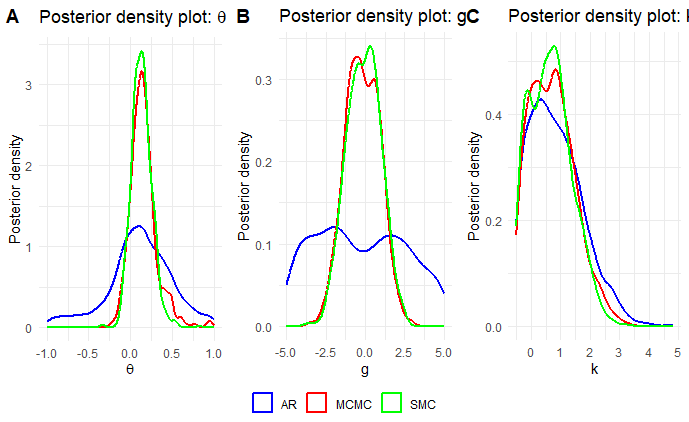
\includegraphics[width=340pt, height=200pt]{Chapters/chapter15/figures/ABCexcrate.png}
	\caption[List of figure caption goes here]{Posterior distributions using approximate Bayesian computation: Exchange rate log returns USD/EURO.}\label{figABCexc}
\end{figure}

\subsection{Bayesian synthetic likelihood}\label{sec15_13}

Note that in ABC, in most cases, we target the posterior distribution $\pi(\boldsymbol{\theta} \mid \boldsymbol{\eta}(\boldsymbol{y}))$ rather than $\pi(\boldsymbol{\theta} \mid \boldsymbol{y})$, as $\boldsymbol{\eta}(\boldsymbol{y})$ is not a sufficient statistic, $\boldsymbol{y}\in \mathbb{R}^N$, $\boldsymbol{\theta}\in \mathbb{R}^K, \ \boldsymbol{\eta}(\boldsymbol{y})\in \mathbb{R}^L, \ L\geq K$. This can be beneficial since discarding information may improve the behavior of the likelihood or make the inference more robust to model misspecification \cite{price2018bayesian}. Given the intractability of $p(\boldsymbol{y} \mid \boldsymbol{\theta})$, it is highly likely that $p(\boldsymbol{\eta}(\boldsymbol{y}) \mid \boldsymbol{\theta})$ is also intractable. \cite{wood2010statistical} addressed this issue by introducing an auxiliary model for the summary statistics, assuming $p_a(\boldsymbol{\eta}(\boldsymbol{y})\mid \boldsymbol{\theta}) = N(\boldsymbol{\mu}_{\boldsymbol{\theta}}, \boldsymbol{\Sigma}_{\boldsymbol{\theta}})$.

Bayesian synthetic likelihood (BSL) arises when this auxiliary likelihood is combined with a prior distribution on the parameter \cite{drovandi2015bayesian,price2018bayesian},
\begin{align*} 
	\pi_{a}(\boldsymbol{\theta} \mid \boldsymbol{\eta}(\boldsymbol{y})) &\propto p_{a}(\boldsymbol{\eta}(\boldsymbol{y})\mid \boldsymbol{\theta}) \pi(\boldsymbol{\theta}), 
\end{align*}

where the subscript \( a \) indicates that this is an approximation due to the Gaussian assumption. This is referred to as the idealized BSL posterior. However, note that \( p_a(\boldsymbol{\eta}(\boldsymbol{y})\mid \boldsymbol{\theta}) \) is rarely available, as \( \boldsymbol{\mu}_{\boldsymbol{\theta}} \) and \( \boldsymbol{\Sigma}_{\boldsymbol{\theta}} \) are generally unknown. Therefore, we estimate these quantities using simulations from the model, following the same steps as in ABC:\footnote{There are better ways to calculate the covariance matrix, see \cite{nott2023bayesian}.}
\begin{align*} 
	\widehat{\boldsymbol{\mu}}_{\boldsymbol{\theta}} &= \frac{1}{M} \sum_{m=1}^{M} \boldsymbol{\eta}(\boldsymbol{z}^{(m)}),\\
	\widehat{\boldsymbol{\Sigma}}_{\boldsymbol{\theta}} &= \frac{1}{M-1} \sum_{m=1}^{M} (\boldsymbol{\eta}(\boldsymbol{z}^{(m)}) - \widehat{\boldsymbol{\mu}}_{\boldsymbol{\theta}})(\boldsymbol{\eta}(\boldsymbol{z}^{(m)}) - \widehat{\boldsymbol{\mu}}_{\boldsymbol{\theta}})^{\top}. 
\end{align*}

Then, we have 
\begin{align*} 
	\pi_{a,M}(\boldsymbol{\theta} \mid \boldsymbol{\eta}(\boldsymbol{y})) &\propto p_{a,M}(\boldsymbol{\eta}(\boldsymbol{y})\mid \boldsymbol{\theta}) \pi(\boldsymbol{\theta}), 
\end{align*}
where $p_{a,M}(\boldsymbol{\eta}(\boldsymbol{y}))$ uses the estimates, which in turn depends on the number of draws $M$ to calculate $\widehat{\boldsymbol{\mu}}_{\boldsymbol{\theta}}$ and $\widehat{\boldsymbol{\Sigma}}_{\boldsymbol{\theta}}$. Note that although we can have unbiased estimators of these object, in general, $N(\boldsymbol{\eta}(\boldsymbol{y})\mid \widehat{\boldsymbol{\mu}}_{\boldsymbol{\theta}},\widehat{\boldsymbol{\Sigma}}_{\boldsymbol{\theta}})$ is not an unbiased estimator of $N(\boldsymbol{\eta}(\boldsymbol{y})\mid {\boldsymbol{\mu}}_{\boldsymbol{\theta}},{\boldsymbol{\Sigma}}_{\boldsymbol{\theta}})$. \cite{an2022bsl} show an unbiased estimator for BSL. 

\cite{nott2023bayesian} show that \( \pi_{a,M}(\boldsymbol{\theta}) \) converges asymptotically to a Gaussian distribution and that the \( 100(1-\alpha)\% \) Bayesian credible regions using BSL have frequentist coverage of \( 100(1-\alpha)\% \). In addition, the posterior mean from BSL is also asymptotically Gaussian. These results require convenient estimation of the covariance matrix and that \( M \to \infty \) as \( N \to \infty \), $M=C\lfloor N^{\gamma} \rfloor, \ C>0, \ \gamma > 0$ and $\lfloor x \rfloor$ denoting the integer floor of $x$. Thus, the choice of \( M \) does not drastically affect the desirable asymptotic properties of BSL \cite{nott2023bayesian}. In addition, \cite{price2018bayesian} find in their examples that posterior inference depends only weakly on \( M \). Thus, \( M \) can be chosen to balance computational efficiency such that the standard deviation of the log synthetic likelihood is between 1 and 3 \cite{an2019accelerating}. 

A critical aspect of BSL is the estimation of the covariance matrix, which can be computationally demanding in high-dimensional settings. However, \cite{nott2023bayesian} propose an adjusted approach to BSL that allows the use of a simple, though potentially misspecified, estimator of the covariance matrix (see Equation 5 and the related discussion in their paper for details).

If the normality assumption for summary statistics is too restrictive, \cite{an2020robust} propose a robust BSL method based on a semi-parametric approach. Additionally, \cite{frazier2021robust} show that when the model is misspecified, i.e., there is no compatibility between the assumed statistical model and the true data-generating process, BSL can lead to unreliable parameter inference. To address this issue, they propose a new BSL method that detects model misspecification and provides more reliable inference.

We can perform BSL using the Algorithm \ref{BSL0}. We can use a random walk Metropolis-Hastings to set the proposal distribution. The covariance matrix of the random walk proposal can be tuned using an initial pilot run.

\begin{algorithm}
	\caption{Bayesian synthetic likelihood}\label{BSL0}
	\begin{algorithmic}[1]
		\For{\texttt{$s=1,\dots,S$}}
			\State Draw $\boldsymbol{\theta}^c\sim q(\boldsymbol{\theta}\mid \boldsymbol{\theta}^{s-1})$
			\For{\texttt{$m=1,\dots,M$}}
				\State Simulate ${\boldsymbol z}^{m}=(z_{1}^{m},z_{2}^{m},...,z_{m}^{s})^{\top}$ from the model, $p(\cdot|{\boldsymbol{\theta} }^c)$
				\State Calculate $\boldsymbol{\eta}(\boldsymbol{z}^{(m)})$
			\EndFor 			 
			\State Calculate $\boldsymbol{\mu}_{\boldsymbol{\theta}^c}$ and $\boldsymbol{\Sigma}_{\boldsymbol{\theta}^c}$
			\State Compute $p_a^c(\boldsymbol{\eta}(\boldsymbol{y})\mid \boldsymbol{\theta}^c) = N(\boldsymbol{\mu}_{\boldsymbol{\theta}^c}, \boldsymbol{\Sigma}_{\boldsymbol{\theta}^c})$ and $p_a^{s-1}(\boldsymbol{\eta}(\boldsymbol{y})\mid \boldsymbol{\theta}^{s-1}) = N(\boldsymbol{\mu}_{\boldsymbol{\theta}^{s-1}}, \boldsymbol{\Sigma}_{\boldsymbol{\theta}^{s-1}})$
			\State Compute the acceptance probability
			$$\alpha(\boldsymbol{\theta}^{s-1},\boldsymbol{\theta}^c)=\min\left\{1,\frac{p_a^c(\boldsymbol{\eta}(\boldsymbol{y})\mid \boldsymbol{\theta}^c)\pi(\boldsymbol{\theta}^c)q(\boldsymbol{\theta}^{s-1}\mid \boldsymbol{\theta}^{c})}{p_a^{s-1}(\boldsymbol{\eta}(\boldsymbol{y})\mid \boldsymbol{\theta}^{s-1})\pi(\boldsymbol{\theta}^{s-1})q(\boldsymbol{\theta}^{c}\mid \boldsymbol{\theta}^{s-1})}\right\}$$
			\State Draw $u$ from $U(0,1)$
			\If{$u<\alpha$}
				\State Set $\boldsymbol{\theta}^{s}=\boldsymbol{\theta}^{c}$, $\boldsymbol{\mu}_{\boldsymbol{\theta}^{s}}=\boldsymbol{\mu}_{\boldsymbol{\theta}^c}$ and $\boldsymbol{\Sigma}_{\boldsymbol{\theta}^s}=\boldsymbol{\Sigma}_{\boldsymbol{\theta}^c}$
			\Else
				\State Set $\boldsymbol{\theta}^{s}=\boldsymbol{\theta}^{s-1}$, $\boldsymbol{\mu}_{\boldsymbol{\theta}^{s}}=\boldsymbol{\mu}_{\boldsymbol{\theta}^{s-1}}$ and $\boldsymbol{\Sigma}_{\boldsymbol{\theta}^s}=\boldsymbol{\Sigma}_{\boldsymbol{\theta}^{s-1}}$
			\EndIf  
		\EndFor
	\end{algorithmic}
\end{algorithm}

An advantage of BSL over ABC is that it does not require selecting a tolerance parameter $\epsilon$. Furthermore, BSL is more computationally efficient than ABC when dealing with a high-dimensional vector of summary statistics as the acceptance rate of the former is asymptotically non-vanishing \cite{nott2023bayesian}.  

On the other hand, ABC is asymptotically more efficient than BSL, and it imposes very weak requirements on the choice of summary statistics, whereas BSL requires summary statistics that satisfy central limit theorems (CLTs), and consistent estimators of the covariance matrix. However, asymptotically, both approaches are equivalent, provided their respective requirements are met \cite{martin2024approximating}.  

In practice, BSL may be more convenient than ABC when the summary statistics are high-dimensional and satisfy CLT conditions. Otherwise, ABC may be the better alternative.\\    

\textbf{Example: Simulation exercise}

We simulate a dataset following the specification of the g-and-k distribution for the financial returns example, setting $\theta_1 = 0.8$, $a = 1$, $b = 0.5$, $g = -1$, and $k = 1$, with a sample size of 500. We use the same priors and summary statistics as in that example.

We use the \textit{BSL} package in \textbf{R} to perform posterior inference using BSL. Additionally, we implement our own BSL sampler to compare the results with the vanilla algorithm from the package. We run the BSL algorithms with $M=200$, $S=11,000$, a burn-in of 1,000, and a thinning parameter of 10, using a random walk proposal distribution. This setting results in similar computational times between the two implementations (scratch and package) and is also comparable to the ABC implementation in Exercise 1.

The following code demonstrates this procedure. The summary statistics appear to be approximately normally distributed, as shown in Figure \ref{figDensSum}, where the red line represents the normal density and the black line represents the estimated density of the summary statistic. Figure \ref{figBSL} displays the posterior distributions from both algorithms for $\theta_1$, $g$, and $k$. In general, the 95\% credible intervals encompass the true parameter values. However, the posterior draws from the \textit{BSL} package are more informative compared to our implementation of Algorithm \ref{BSL0}. Additionally, BSL outperforms the results of ABC in Exercise 1, yielding more precise posterior distributions. This pattern has been observed in other settings \cite{drovandi2022comparison,martin2024approximating}. Both ABC and BSL produce posterior distributions centered at the true parameter values, although the posterior distribution of $\theta_1$ deviates from this pattern.

\begin{tcolorbox}[enhanced,width=4.67in,center upper,
	fontupper=\large\bfseries,drop shadow southwest,sharp corners]
	\textit{R code. g-and-k simulation: Bayesian synthetic likelihood}
	\begin{VF}
		\begin{lstlisting}[language=R]
######## BSL: g-and-k simulation ############
rm(list = ls()); set.seed(010101); library(BSL)
# Simulate g-and-k data
RGKnew <- function(par) {
	z <- NULL
	theta <- par[1]; a <- par[2]; b <- par[3]; g <- par[4]; k <- par[5]
	e <- rnorm(n + 1)
	for(t in 2:(n + 1)){
		zt <- e[t] + theta * e[t-1]
		z <- c(z, zt)
	}
	zs <- z / (1 + theta^2)^0.5
	x <- a + b * (1 + 0.8 * (1 - exp(-g * zs)) / (1 + exp(-g * zs))) * (1 + zs^2)^k * zs
	return(x)
}
# Summary statistics
SumSt <- function(y) {
	Oct <- quantile(y, c(0.125, 0.25, 0.375, 0.5, 0.625, 0.75, 0.875))
	eta1 <- Oct[6] - Oct[2]
	eta2 <- (Oct[6] + Oct[2] - 2 * Oct[4]) / eta1
	eta3 <- (Oct[7] - Oct[5] + Oct[3] - Oct[1]) / eta1
	autocor <- acf(y, lag = 2, plot = FALSE)
	autocor[["acf"]][2:3]
	Etay <- c(Oct, eta1, eta2, eta3, autocor[["acf"]][2:3])
	return(Etay)
}
# Prior function
LogPrior <- function(par){
	LogPi <- log(par[1] > -1 & par[1] < 1 & par[2] > 0 & par[2] < 5 & par[3] > 0 & par[3] < 5 & par[4] > -5 & par[4] < 5 & par[5] > -0.5 & par[5] < 5)
	return(LogPi)
}
# Population parameters
theta1 <- 0.8; a <- 1; b <- 0.5; g <- -1; k <- 1
parpop <- c(theta1, a, b, g, k)
K <- 5
n <- 500
y <- RGKnew(par = parpop)
# Algorithm parameters
M <- 200 # Number of iterations to calculate mu and sigma
S <- 11000 # Number of MCMC iterations
burnin <- 1000 # Burn in iterations
thin <- 10 # Thining parameter
keep <- seq(burnin + 1, S, thin)
par0 <- c(0.5, 2, 1, 0, 1) 
Modelgk <- newModel(fnSim = RGKnew, fnSum = SumSt, theta0 = par0, fnLogPrior = LogPrior, verbose = FALSE)
validObject(Modelgk)
# Check if the summary statistics are roughly normal
simgk <- simulation(Modelgk, n = M, theta = par0, seed = 10)
par(mfrow = c(4, 3))
\end{lstlisting}
	\end{VF}
\end{tcolorbox}

\begin{tcolorbox}[enhanced,width=4.67in,center upper,
	fontupper=\large\bfseries,drop shadow southwest,sharp corners]
	\textit{R code. g-and-k simulation: Bayesian synthetic likelihood}
	\begin{VF}
		\begin{lstlisting}[language=R]
for (i in 1:12){
	eval <- seq(min(simgk$ssx[, i]), max(simgk$ssx[, i]), 0.001)
	densnorm <- dnorm(eval, mean = mean(simgk$ssx[, i]), sd(simgk$ssx[, i])) 
	plot(density(simgk$ssx[, i]), main = "", xlab = "")
	lines(eval, densnorm, col = "red")
}
##### Program from scratch #######
Lims <- matrix(c(-1, 0, 0, -5, -0.5, 1, rep(5, 4)), 5, 2)
parPost <- matrix(NA, S, K); parPost[1,] <- par0 ; EtaY <- SumSt(y = y)
Zsl <- replicate(M, RGKnew(par = parPost[1,]))
EtasZsl <- t(apply(Zsl, 2, SumSt))
Usl <- colMeans(EtasZsl); SIGMAsl <- var(EtasZsl)
dnormsl <- mvtnorm::dmvnorm(EtaY, Usl, SIGMAsl, log = TRUE)
tune <- 0.005; CoVarRW <- tune*diag(K)
accept <- rep(0, S); tick1 <- Sys.time()
pb <- winProgressBar(title = "progress bar", min = 0, max = S, width = 300)
for (s in 2:S){
	parc <- MASS::mvrnorm(1, mu = parPost[s-1,], Sigma = CoVarRW)
	RestCheck <- NULL
	for(j in 1:K){
		if(parc[j] < Lims[j,1] | parc[j] > Lims[j,2]){
			Rej <- 1
		}else{Rej <- 0}
		RestCheck <- c(RestCheck, Rej)
	}
	if(sum(RestCheck) != 0){
		parPost[s,] <- parPost[s-1,]; accept[s] <- 0
	}else{
		Z <- replicate(M, RGKnew(par = parc))
		EtasZ <- t(apply(Z, 2, SumSt))
		Um <- colMeans(EtasZ); SIGMAm <- var(EtasZ)
		dnormc <- mvtnorm::dmvnorm(EtaY, Um, SIGMAm, log = TRUE)
		if(s > round(0.1*S, 0) & s < round(0.2*S, 0)){
			CoVarRW <- var(parPost, na.rm = TRUE)
		}
		if(dnormc == -Inf){
			parPost[s,] <- parPost[s-1,]; accept[s] <- 0
		}else{
			alpha <- min(1, exp(dnormc - dnormsl)); U <- runif(1)
			if(U <= alpha){
				parPost[s,] <- parc; Usl <- Um; SIGMAsl <- SIGMAm
				dnormsl <- dnormc; accept[s] <- 1
			}else{
				parPost[s,] <- parPost[s-1,]; accept[s] <- 0
			}
		}
	}
	setWinProgressBar(pb, s, title=paste( round(s/S*100, 0),"% done"))
}
\end{lstlisting}
	\end{VF}
\end{tcolorbox}

\begin{tcolorbox}[enhanced,width=4.67in,center upper,
	fontupper=\large\bfseries,drop shadow southwest,sharp corners]
	\textit{R code. g-and-k simulation: Bayesian synthetic likelihood}
	\begin{VF}
		\begin{lstlisting}[language=R]
close(pb); tock1 <- Sys.time(); tock1 - tick1
mean(accept)
PostChainOwn <- coda::mcmc(parPost[keep,])
summary(PostChainOwn)
#### BSL package
tick <- Sys.time()
Resultsgk <- bsl(y = y, n = M, M = S, model = Modelgk, covRandWalk = CoVarRW,
method = "BSL", thetaNames = expression(theta, a, b, g, k), plotOnTheFly = TRUE)
tock <- Sys.time(); tock - tick
PostChain <- coda::mcmc(Resultsgk@theta[keep,])
summary(PostChain)
Resultsgk@acceptanceRate
plot(Resultsgk@loglike[keep], type = "l")
sd(Resultsgk@loglike[keep])
# Figures 
library(ggplot2); library(latex2exp)
Sp <- length(keep)
df1 <- data.frame(Value = c(PostChain[,1], PostChainOwn[,1]), Distribution = factor(c(rep("BSL", Sp), rep("BSLscratch", Sp))))
dentheta <- ggplot(df1, aes(x = Value, color = Distribution)) + geom_density(linewidth = 1) + labs(title = TeX("Posterior density plot: $theta$"), x = TeX("$theta$"), y = "Posterior density") + geom_vline(xintercept = theta1, linetype = "dashed", color = "red", linewidth = 1) + scale_color_manual(values = c("blue", "red")) +  theme_minimal() +
theme(legend.title = element_blank())
df2 <- data.frame(Value = c(PostChain[,4], PostChainOwn[,4]), Distribution = factor(c(rep("BSL", Sp), rep("BSLscratch", Sp))))
deng <- ggplot(df2, aes(x = Value, color = Distribution)) + geom_density(linewidth = 1) + labs(title = "Posterior density plot: g", x = "g", y = "Posterior density") +
geom_vline(xintercept = g, linetype = "dashed", color = "red", linewidth = 1) +
scale_color_manual(values = c("blue", "red")) + theme_minimal() + theme(legend.title = element_blank())
df3 <- data.frame(Value = c(PostChain[,5], PostChainOwn[,5]), Distribution = factor(c(rep("BSL", Sp), rep("BSLscratch", Sp))))
denk <- ggplot(df3, aes(x = Value, color = Distribution)) +   geom_density(linewidth = 1) + labs(title = "Posterior density plot: k", x = "k", y = "Posterior density") + geom_vline(xintercept = k, linetype = "dashed", color = "red", linewidth = 1) + scale_color_manual(values = c("blue", "red")) +  theme_minimal() + theme(legend.title = element_blank())
library(ggpubr)
ggarrange(dentheta, deng, denk, labels = c("A", "B", "C"), ncol = 3, nrow = 1,
legend = "bottom", common.legend = TRUE)
\end{lstlisting}
	\end{VF}
\end{tcolorbox}

\begin{figure}[!h]
	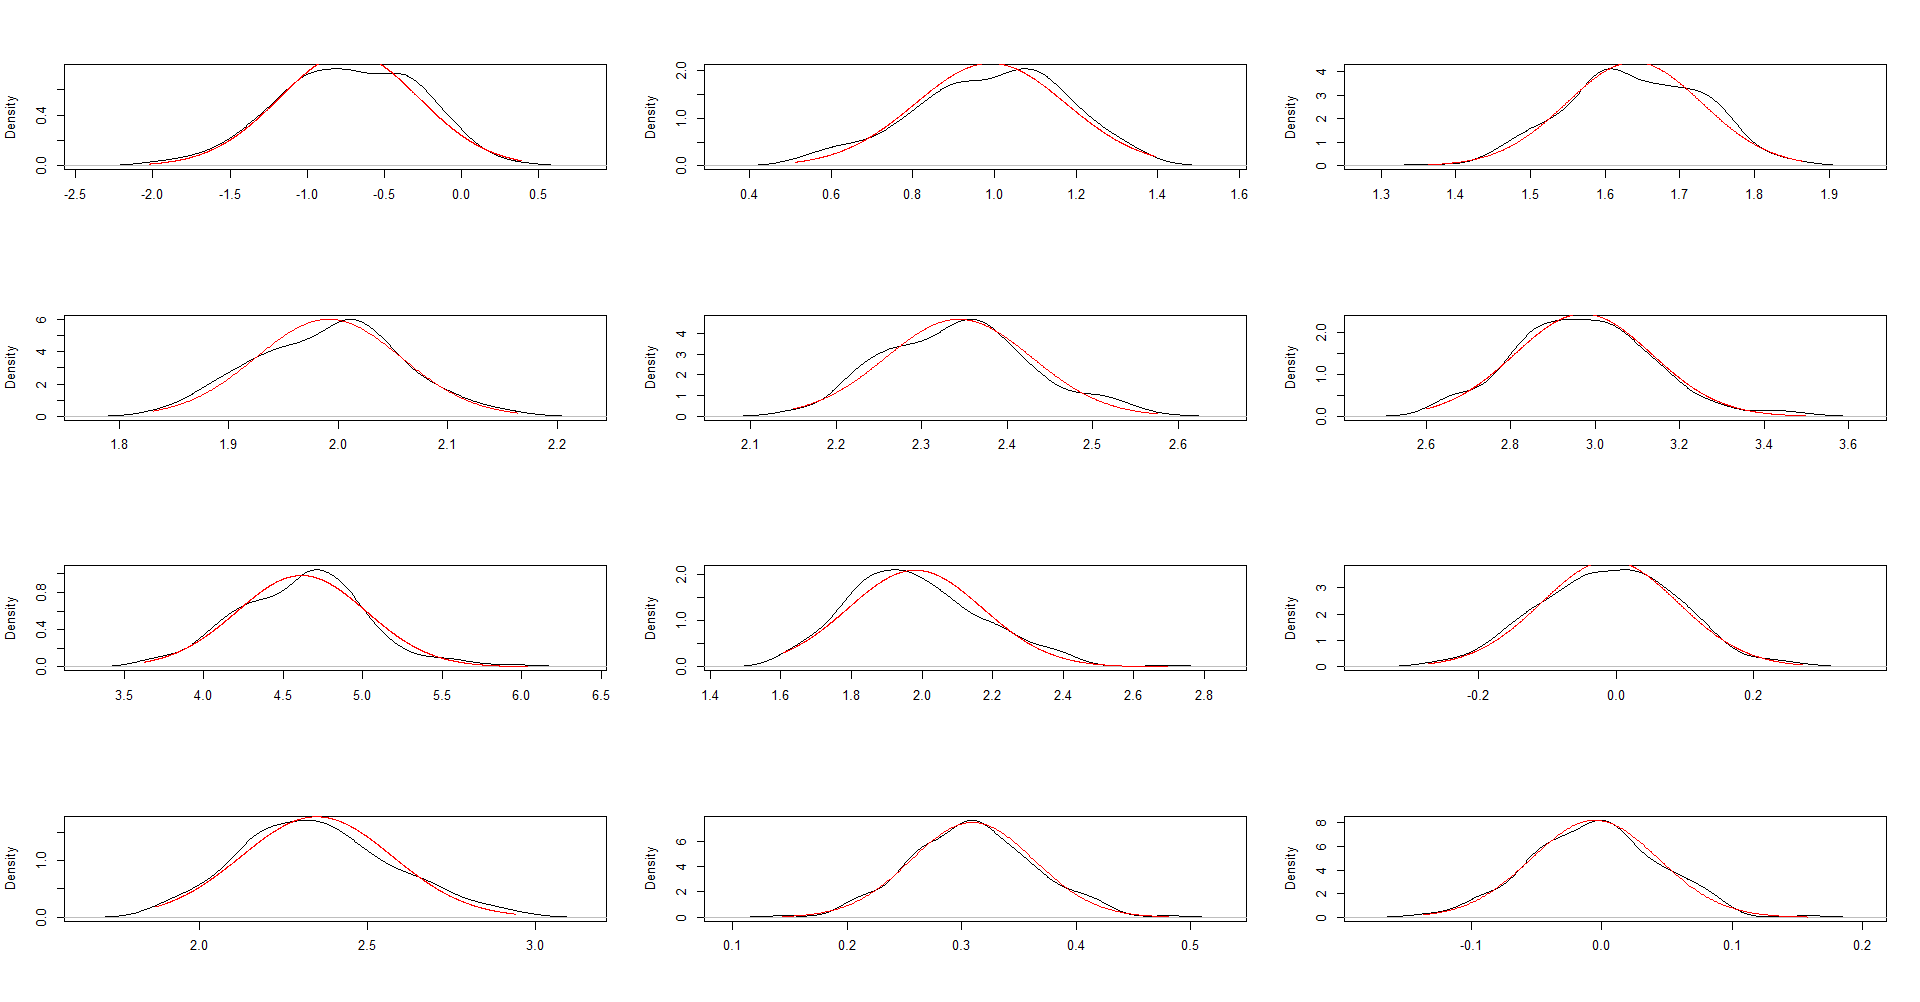
\includegraphics[width=340pt, height=200pt]{Chapters/chapter15/figures/DensitiesSum.png}
	\caption[List of figure caption goes here]{Density estimates of summary statistics: g-and-k simulation.}\label{figDensSum}
\end{figure} 

\begin{figure}[!h]
	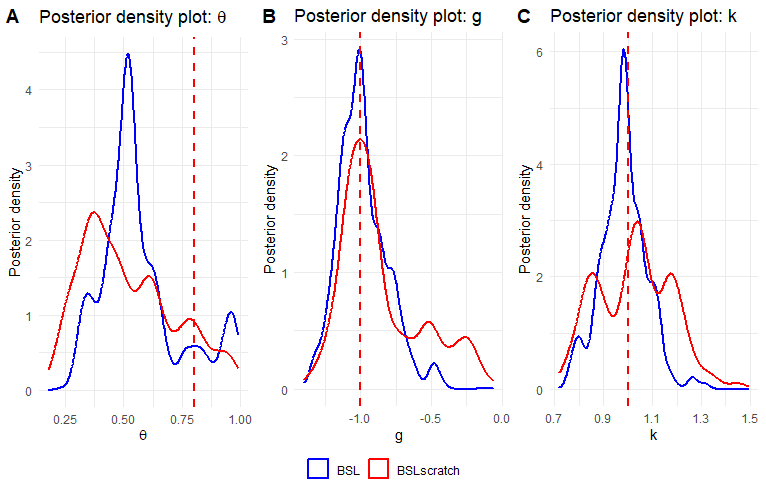
\includegraphics[width=340pt, height=200pt]{Chapters/chapter15/figures/BSLgksim.png}
	\caption[List of figure caption goes here]{Posterior distributions using Bayesian synthetic likelihood: g-and-k simulation.}\label{figBSL}
\end{figure}


\section{Optimization approaches}\label{sec15_2}

MCMC and IS algorithms require pointwise evaluation of the likelihood function, which implies a massive number of operations when dealing with very large datasets. Unfortunately, these algorithms are not designed to be \textit{scalable}. Moreover, if the parameter space is large, these methods are also not \textit{scalable} in the number of parameters. Therefore, approximation methods should be used even when the likelihood function has an analytical expression.

\textit{Optimization approaches} are designed to scale to high parameter spaces and large datasets. The trick is to change simulation with optimization. 

\subsection{Integrated nested Laplace approximations}\label{sec15_21}
\textit{Integrated nested Laplace approximations} approximates $\pi(\boldsymbol{\theta} \mid \mathbf{y})$ by a combination of low-dimensional deterministic integration and optimization steps. 

\subsection{Variational Bayes}\label{sec15_22}
\textit{Variational Bayes} (VB) is a method from machine learning \cite{jordan1999introduction,wainwright2008graphical} that replaces $\pi(\boldsymbol{\theta} \mid \mathbf{y})$ by an approximation produced by optimization using calculus of variations, that is why the method is called \textit{variational} Bayes. This can happen because the posterior distribution is very complicated, for instance multimodal, or there is a high-dimensional problem that would take too long to solve using MCMC or IS algorithms. 

Thus, the aim in VB is to approximate the posterior distribution using $q(\boldsymbol{\theta})$ that belongs to the variational family $\mathcal{Q}$, where this should be a family of distributions that would be computationally easy to work with, but flexible enough to get a good approximation of the posterior distribution \cite{blei2017variational}. Then, $q$ is called the \textit{variational approximation} to the posterior distribution, and a particular $q$ in $\mathcal{Q}$ is specified by obtaining a particular set of \textit{variational parameters}. This is commonly performed minimizing the Kullback-Leibler divergence between $q(\boldsymbol{\theta})$ and $\pi(\boldsymbol{\theta} \mid \mathbf{y})$,
\begin{align}\label{eq:VB1}
	q^*(\boldsymbol{\theta}):=\underset{q \in \mathcal{Q}}{\argmin} \  \text{KL}(q(\boldsymbol{\theta})||\pi(\boldsymbol{\theta} \mid \mathbf{y})),
\end{align}  
where $\text{KL}(q(\boldsymbol{\theta})||\pi(\boldsymbol{\theta} \mid \mathbf{y}))=\mathbb{E}_q\left[\log\left(\frac{q(\boldsymbol{\theta})}{\pi(\boldsymbol{\theta} \mid \mathbf{y})}\right)\right]$.\footnote{The Kullback-Leibler divergence, also known as the relative entropy, is non-negative, equal 0 when $q(\boldsymbol{\theta})=\pi(\boldsymbol{\theta} \mid \mathbf{y})$, otherwise is positive. However, it does not satisfy the triangular inequality nor is symmetric, that is, $\text{KL}(q(\boldsymbol{\theta})||\pi(\boldsymbol{\theta} \mid \mathbf{y}))\neq \text{KL}(\pi(\boldsymbol{\theta} \mid \mathbf{y})||q(\boldsymbol{\theta}))$, that is why it is not a distance (metric).} 

Note that in relatively complex models the optimization in \ref{eq:VB1}  is not computable due to depending on the marginal likelihood $p(\boldsymbol{y})$, which is normally unknown due to the implicit integral does not have analytical solution. However, there is a solution to this situation. Let's see,
\begin{align*}
	\log(p(\boldsymbol{y}))&=\log\left(\int_{\boldsymbol{\Theta}}p(\boldsymbol{y}\mid \boldsymbol{\theta})\pi(\boldsymbol{\theta})d\boldsymbol{\theta}\right)\\
	&=\log\left(\int_{\boldsymbol{\Theta}}p(\boldsymbol{y}, \boldsymbol{\theta})d\boldsymbol{\theta}\right)\\
	&=\log\left(\int_{\boldsymbol{\Theta}}\frac{p(\boldsymbol{y}, \boldsymbol{\theta})}{q(\boldsymbol{\theta})}q(\boldsymbol{\theta})d\boldsymbol{\theta}\right)\\
	&=\log \mathbb{E}_q\left(\frac{p(\boldsymbol{y}, \boldsymbol{\theta})}{q(\boldsymbol{\theta})}\right)\\
	&\geq \mathbb{E}_q\log\left(\frac{p(\boldsymbol{y}, \boldsymbol{\theta})}{q(\boldsymbol{\theta})}\right)\\
	&=\mathbb{E}_q\log(p(\boldsymbol{y}, \boldsymbol{\theta}))-\mathbb{E}_q\log(q(\boldsymbol{\theta}))\\
	&=\text{ELBO}(q(\boldsymbol{\theta})),
\end{align*}
where the inequality is from the Jensen's inequality, and $\log(\cdot)$ is concave. The last term is the evidence lower bound (ELBO), which is a lower bound of the marginal likelihood.
Note that the gap between the marginal likelihood and the ELBO is given by
\begin{align*}
	\log(p(\boldsymbol{y})) - \text{ELBO}(q(\boldsymbol{\theta})) & = \log(p(\boldsymbol{y})) - \mathbb{E}_q\log(p(\boldsymbol{y}, \boldsymbol{\theta}))+\mathbb{E}_q\log(q(\boldsymbol{\theta}))\\
	&=\mathbb{E}_q\left(\log(q(\boldsymbol{\theta}))-\log\left(\frac{p(\boldsymbol{y}, \boldsymbol{\theta})}{p(\boldsymbol{y})}\right)\right)\\
	&=\mathbb{E}_q\left(\log(q(\boldsymbol{\theta}))-\log\left(\frac{p(\boldsymbol{y}\mid \boldsymbol{\theta})\pi( \boldsymbol{\theta})}{p(\boldsymbol{y})}\right)\right)\\
	&=\mathbb{E}_q\left(\log(q(\boldsymbol{\theta}))-\log(\pi(\boldsymbol{\theta}\mid \boldsymbol{y}))\right)\\
	&=\text{KL}(q(\boldsymbol{\theta})||\pi(\boldsymbol{\theta} \mid \mathbf{y})).	 
\end{align*}
Then,
\begin{align*}
	\log(p(\boldsymbol{y})) = \text{KL}(q(\boldsymbol{\theta})||\pi(\boldsymbol{\theta} \mid \mathbf{y})) + \text{ELBO}(q(\boldsymbol{\theta})),  
\end{align*} 
which implies that maximizing the ELBO with respect to $q(\boldsymbol{\theta})$ implies minimizing the KL divergence due to $\log(p(\boldsymbol{y}))$ does not depend on $q(\boldsymbol{\theta})$. This avoids calculating the marginal likelihood, and consequently is easier to solve the variational problem. In addition, it gives a lower bound for the marginal likelihood, which potentially can be used for model choice. Thus, the solution of the problem \ref{eq:VB1} is equivalent to solve
\begin{align}\label{eq:VB2}
	q^*(\boldsymbol{\theta}):=\underset{q \in \mathcal{Q}}{\argmax} \  \text{ELBO}(q(\boldsymbol{\theta})).
\end{align}

Note that the ELBO can be also expressed as 
\begin{align*}
	\text{ELBO}(q(\boldsymbol{\theta}))&=\mathbb{E}_q\log(p(\boldsymbol{y}, \boldsymbol{\theta}))-\mathbb{E}_q\log(q(\boldsymbol{\theta}))\\
	&=\mathbb{E}_q\log(p(\boldsymbol{y}\mid \boldsymbol{\theta}))+\mathbb{E}_q\log(\pi(\boldsymbol{\theta}))-\mathbb{E}_q\log(q(\boldsymbol{\theta}))\\
	&=\mathbb{E}_q\log(p(\boldsymbol{y}\mid \boldsymbol{\theta}))-\text{KL}(q(\boldsymbol{\theta})||\pi(\boldsymbol{\theta})).
\end{align*} 
This means that when maximizing the ELBO, we look for $\boldsymbol{\theta}$ that maximizes the likelihood, and minimizes the KL divergence between the variational distribution and the prior. Thus, we are looking for a balance between the prior and the likelihood, which is what we do when obtaining the posterior distribution.

The most common approach to set $q(\boldsymbol{\theta})$ is assuming independence in some blocks of $\boldsymbol{\theta}$, that is, $q(\boldsymbol{\theta})=\prod_{l=1}^K q_l(\boldsymbol{\theta}_l)$. This is called the mean-field variational family, the name comes from statistical physics. Each $q_l(\boldsymbol{\theta}_l)$ is function of a set of \textit{variational parameters}, and optimization is with respect to them. Note that the mean-field approximation does not capture dependencies between the parameters; although, it can capture the marginal densities.

Let's decompose the ELBO under the mean-field variational family \cite{nguyen2023depth},
\begin{align*}
		\text{ELBO}(q(\boldsymbol{\theta}))&=\mathbb{E}_q\log(p(\boldsymbol{y}, \boldsymbol{\theta}))-\mathbb{E}_q\log(q(\boldsymbol{\theta}))\\
	&=\int_{\mathbb{R}^L} \log(p(\boldsymbol{y}, \boldsymbol{\theta}))q(\boldsymbol{\theta})d\boldsymbol{\theta}-\int_{\mathbb{R}^L}\log(q(\boldsymbol{\theta}))q(\boldsymbol{\theta})d\boldsymbol{\theta}\\
	&=\int_{\mathbb{R}^L} \log\left(p(\boldsymbol{y}, \boldsymbol{\theta})\right)\prod_{l=1}^K q_l(\boldsymbol{\theta}_l)d\boldsymbol{\theta}_l-\int_{\mathbb{R}^L}\log\left(\prod_{l=1}^K q_l(\boldsymbol{\theta}_l)\right)\prod_{l=1}^K q_l(\boldsymbol{\theta}_l)d\boldsymbol{\theta}_l\\
	&=\int_{\mathbb{R}} \underbrace{\left(\int_{\mathbb{R}^{K-1}}\log\left(p(\boldsymbol{y}, \boldsymbol{\theta})\right)\prod_{l\neq k} q_l(\boldsymbol{\theta}_l)d\boldsymbol{\theta}_l\right)}_{\mathbb{E}_{-k}(\log\left(p(\boldsymbol{y}, \boldsymbol{\theta})\right))}q_k(\boldsymbol{\theta}_k)d\boldsymbol{\theta}_k\\ 
	&-\int_{\mathbb{R}}\log(q_k(\boldsymbol{\theta}_k))q_k(\boldsymbol{\theta}_k)d\boldsymbol{\theta}_k-\sum_{l\neq k}\int_{\mathbb{R}}\log(q_l(\boldsymbol{\theta}_l))q_l(\boldsymbol{\theta}_l)d\boldsymbol{\theta}_l\\
	&=\int_{\mathbb{R}}\log\left\{\exp\left(\mathbb{E}_{-k}(\log\left(p(\boldsymbol{y}, \boldsymbol{\theta})\right))\right)\right\}q_k(\boldsymbol{\theta}_k)d\boldsymbol{\theta}_k\\ 
	&-\int_{\mathbb{R}}\log(q_k(\boldsymbol{\theta}_k))q_k(\boldsymbol{\theta}_k)d\boldsymbol{\theta}_k-\sum_{l\neq k}\int_{\mathbb{R}}\log(q_l(\boldsymbol{\theta}_l))q_l(\boldsymbol{\theta}_l)d\boldsymbol{\theta}_l\\
	&=\int_{\mathbb{R}}\log\left\{\frac{\exp\left(\mathbb{E}_{-k}(\log\left(p(\boldsymbol{y}, \boldsymbol{\theta})\right))\right)}{q_k(\boldsymbol{\theta}_k)}\right\}q_k(\boldsymbol{\theta}_k)d\boldsymbol{\theta}_k\\
	&-\sum_{l\neq k}\int_{\mathbb{R}}\log(q_l(\boldsymbol{\theta}_l))q_l(\boldsymbol{\theta}_l)d\boldsymbol{\theta}_l\\ 
	&=-\text{KL}(q_k(\boldsymbol{\theta}_k)||\exp\left(\mathbb{E}_{-k}(\log\left(p(\boldsymbol{y}, \boldsymbol{\theta})\right))\right))-\sum_{l\neq k}\int_{\mathbb{R}}\log(q_l(\boldsymbol{\theta}_l))q_l(\boldsymbol{\theta}_l)d\boldsymbol{\theta}_l\\
	&\leq -\sum_{l\neq k}\int_{\mathbb{R}}\log(q_l(\boldsymbol{\theta}_l))q_l(\boldsymbol{\theta}_l)d\boldsymbol{\theta}_l,
\end{align*} 
where $\mathbb{E}_{-k}$ denotes expectation with respect to the distribution $\prod_{l\neq k}q(\boldsymbol{\theta}_l)$.

Note that we maximize the ELBO when $\text{KL}(q_k(\boldsymbol{\theta}_k)||\exp\left(\mathbb{E}_{-k}(\log\left(p(\boldsymbol{y}, \boldsymbol{\theta})\right))\right))$ equals 0, that is, when
\begin{align}\label{eq:VB3}
	q_k^*(\boldsymbol{\theta}_k)&\propto\exp\left(\mathbb{E}_{-k}(\log\left(p(\boldsymbol{y}, \boldsymbol{\theta})\right))\right)\\
	&=\exp\left(\mathbb{E}_{-k}(\log\left(p(\boldsymbol{y}, \boldsymbol{\theta}_{-k},\boldsymbol{\theta}_k)\right))\right)\\
	&=\exp\left(\mathbb{E}_{-k}(\log\left(p({\boldsymbol{\theta}}_{k}\mid\boldsymbol{y},\boldsymbol\theta_{-k})p(\boldsymbol{y},\boldsymbol\theta_{-k})\right))\right)\\
	&\propto \exp\left(\mathbb{E}_{-k}(\log\left(p(\boldsymbol{\theta}_{k}\mid\boldsymbol{y},\boldsymbol\theta_{-k})\right))\right), k=1,2,\dots,L.
\end{align}

Note the circular dependency nature of $q_k^*(\boldsymbol{\theta}_k)$, that is, $q_k^*(\boldsymbol{\theta}_k)$ depend on $q_{-k}^*(\boldsymbol{\theta}_{-k})$ (see example belong for clarity). Thus, there is need to solve this situation algorithmically. Probably, one of the most common algorithm to solve the optimization problem in \ref{eq:VB2} using \ref{eq:VB3} is coordinate ascent variational inference (CAVI) \cite{bishop2006pattern}. The algorithm departs from an initial solution, and then, cycles through $q_k^*(\boldsymbol{\theta}_k), k=1,2,\dots,L$ updating each component in turn. Algorithm \ref{VB0} shows the basis of the CAVI algorithm. 

\begin{algorithm}
	\caption{Variational Bayes: Coordinate ascent variational inference}\label{VB0}
	\begin{algorithmic}[1]
		\State Initialize the variational factors $q_l^*(\boldsymbol{\theta}_l), l=1,2,\dots,K$
		\While{ELBO $>\epsilon$, $\epsilon$ small} 
			\For{$l=1,2,\dots,L$} 
				\State Set $q_l^*(\boldsymbol{\theta}_l)\propto \exp\left(\mathbb{E}_{-l}(\log\left(p({\theta}_{l}\mid\boldsymbol{y},\boldsymbol\theta_{-l})\right))\right)$
			\EndFor
		\State Compute $\text{ELBO}(q)=\mathbb{E}_q\log(p(\boldsymbol{y}, \boldsymbol{\theta}))-\mathbb{E}_q\log(q(\boldsymbol{\theta}))$
		\EndWhile 
		\State Return $q(\boldsymbol{\theta})$ 
	\end{algorithmic}
\end{algorithm}
 
We should say that the CAVI algorithm is sensitive to the initial variational due to the algorithm garanties convergence to a local maximum that can be sensitive to the point of initialization. This issue can be metigated using different initialization points and selecting the one with the highest ELBO \cite{blei2006variational}.

 
Note that the method is deterministic, rather than stochastic, that is, it does not require approximating the posterior distribution by draws from other simpler distributions. This makes VB faster in many cases compared to MCMC methods, which are stochastic. It requires to solve a deterministic optimization problem to find the \textit{best variational distribution} in a particular simple family, normally in the exponential family, by finding the parameters of this distribution such that minimize the KL divergence to the posterior distribution. Once the \textit{variational parameters} are found, we can sample from the simple \textit{variational distribution} to perform estimation, hypothesis testing, prediction, etc.  

Gibbs sampler iterates between random draws of conditional posterior distributions, whereas VB determiniscaly iterates between distributions. Thus, VB works directly with distributions rather than with draws, it is approximate, but faster. The aim in expectation propagation is to minimize $\text{KL}(\pi(\boldsymbol{\theta} \mid \mathbf{y})||q(\boldsymbol{\theta}))$ rather than $\text{KL}(q(\boldsymbol{\theta})||\pi(\boldsymbol{\theta} \mid \mathbf{y}))$.  

VB overestimates the precision of the posterior distribution, but not necessarily suffers in accuracy \cite{blei2017variational}.

\cite{zhang2020convergence} analyzes the asymptotic properties of VB posterior decomposing the convergence rates of VB in the convergence rate of the true posterior and the approximation error induced by the variational family. These authors show that the VB posterior concentrates entirely in a neighborhood of the true posterior distribution. In addition, if the loss function is convex, there exists a point estimator that converges at the same rate. \cite{zhang2020convergence} also show for specific cases, like sparse linear models, the concentration rate of the VB posterior is faster than the concentration rate of the exact posterior.  

\section{Summary}\label{sec15_3}
\textit{Simulation-based algorithms} suffer from the \textit{curse of dimensionality} in parameter space, whereas \textit{Optimization approaches} require evaluation of the likelihood functions. Thus, recent approaches mix these two approaches to overcome situations where both phenomena are present.

\section{Exercises}\label{sec15_4}

\begin{enumerate}
	\item \textbf{g-and-k distribution for financial returns continues I}
	
	Simulate a dataset following the specification given in the g-and-k distribution for financial returns example. Set $\theta_1 = 0.8$, $a = 1$, $b = 0.5$, $g = -1$, and $k = 1$, with a sample size of 500, and use the same priors as in that example. Implement the ABC accept/reject algorithm from scratch using one million prior draws, selecting the 1,000 draws with the smallest distance.\footnote{Note that this setting does not satisfy the asymptotic requirements for Bayesian consistency. However, it serves as a pedagogical exercise.}
	
	\begin{itemize}
		\item Perform a linear regression adjustment using the posterior draws of our ABC-AR algorithm (ABC-AR-Adj).
		\item Compare the results with those obtained using the ABC-AR implementation in the \textit{EasyABC} package, ensuring that the computational time is relatively similar between both implementations.
		\item Compare the posterior results of ABC-AR, ABC-AR-Adj and EasyABC with the population values.
	\end{itemize}
	
	\begin{comment}
	\item Simulate a model $y_i=0.5 x_i+u_i, \ i=1,2,\dots,250$, where 
	
	$$v_i=Q^{gk}\left\{z(p)\mid a_i, b_j, c_j, g_j, k_j\right\}, \  v_j=(x_j,u_j), \ \begin{Bmatrix} z(p_x) \\ z(p_u)\end{Bmatrix}\sim N \begin{Bmatrix} \begin{pmatrix} 0\\ 0\end{pmatrix}, \begin{pmatrix} 1 & 0.5 \\ 0.5 & 1\end{pmatrix} \end{Bmatrix}.$$
	
	Note that in this model there endogeneity as $x_j$ and the stochastic errors ($u_j$) are no independent.
	
	We took into account values for $\rho =\left\{0,0.4,0.8\right\}$, $\rho\neq 0$ implies that inference should be based on the joint likelihood function, $y_{j}=0.5x_j+u_j$ where $a_x=a_u=0$, $b_x=b_u=1$, $c_x=c_u=0.8$, $g_x=g_u=2$, $k_x=k_u=1$, and $n=(500, 1000)$ in 50 simulation exercises. We perform inference regarding $\beta$ and $k$ in this example, and fixed $a, b$ and $g$ at their population values. We consider as the basis of our analysis the summary statistics $\eta_{1}({y})=\sum_{i=1}^{n}x_iy_i/\sum_{i=1}^{n}x_i^2$, $\eta_2({y})=L_3-L_1$, $\eta_3({y})=(L_3+L_1-2L_2)/\eta_2$  and $\eta_4({y})=(E_7-E_5+E_3-E_1)/\eta_2$ where $L_l$ is the $l$th quartile and $E_l$ is the $l$th octile of $y_j-x_j\eta_1({y})$ \cite{drovandi2011likelihood}.
	
	\item Given a Poisson model with parameter $\lambda$ and prior distribution gamma with shape and rate parameters $\alpha_0=\delta_0$ gives a posterior gamma distribution with parameters $\alpha_n=\alpha_0+\sum_{i=1}^N y_i$ and $\delta_n=\delta_0+N$. This model can be interpreted as a Poisson likelihood with unobserved heterogeneity, and gives a likelihood that is negative binomial with number of success $\alpha_n$ and probability $1/(1+\delta_n)$. Perform inference of $\lambda$ using ABC and BSL, and compare the results with the standard closed-form posterior.
	\end{comment}
	\item \textbf{g-and-k distribution for financial returns continues II}
	
	Perform inference in the financial returns example using Bayesian synthetic likelihood, setting $M=500$, $S=11,000$, a burn-in of 1,000, and a thinning parameter of 10. This setting results in a similar computational time to the ABC algorithm. Use a random walk proposal distribution in the \textit{BSL} package in \textbf{R}, and compare the results with those from ABC.  
	
	
\item 
	
\end{enumerate}

